\documentclass[]{article}

%Language settings
\usepackage[spanish]{babel}

%Paper size and margins
\usepackage[letterpaper,top=2.54cm,bottom=2.54cm,left=2.54cm,right=2.54cm,marginparwidth=1.75cm]{geometry}

%Other packages
\usepackage{amsmath}
\usepackage{graphicx}
\usepackage[colorlinks=true, allcolors=blue]{hyperref}

\title{11. Control Reversible de un Motor DC con 3 Botones de Entrada y Velocidad Variable}
\author{Flores Tun, Jorge David; López Gómez, Wilberth Eduardo; Sánchez Soberanis, Felipe}

\begin{document}
\maketitle

\section{Introducción}

Para el giro de un motor en sentido horario y antihorario, se pretende construir un control mediante un puente h, donde intervienen dos relevadores conectados a las terminales
del motor para que este gire en un sentido u otro. De igual manera, los relevadores serán conectados a optoacopladores, los cuales serán controlados por un microcontrolador, en nuestro
caso de una tarjeta PSOC, el cual podrá controlar los pulsos para alimentar al motor. Para la regulación de velocidad, se incorporará un tercer optoacoplador con el fin de conectar 
un potenciómetro que regule el voltaje que llega al motor, afectando en su velocidad.
\section{Marco teórico}

\subsection{Puente H}

Se le denomina puente h al tipo de configuración que permite la activación de motores DC en más de un solo sentido que consiste en 4 interruptores que varían su combinación según 
el usuario desee.

\begin{figure}[htb]
    \centering
    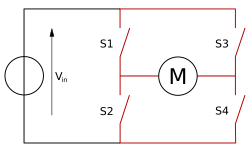
\includegraphics[width=6cm]{Imagenes/H.png}
    \caption{Estructura de un puente H}
\end{figure}

\subsection{Relevador}

 Se le conoce como relevador a un interruptor que es controlado mediante magnetismo y puede ofrecer o suspender la alimantación de un nodo eléctrico a un sistema.
\clearpage
 \begin{figure}[htb]
     \centering
     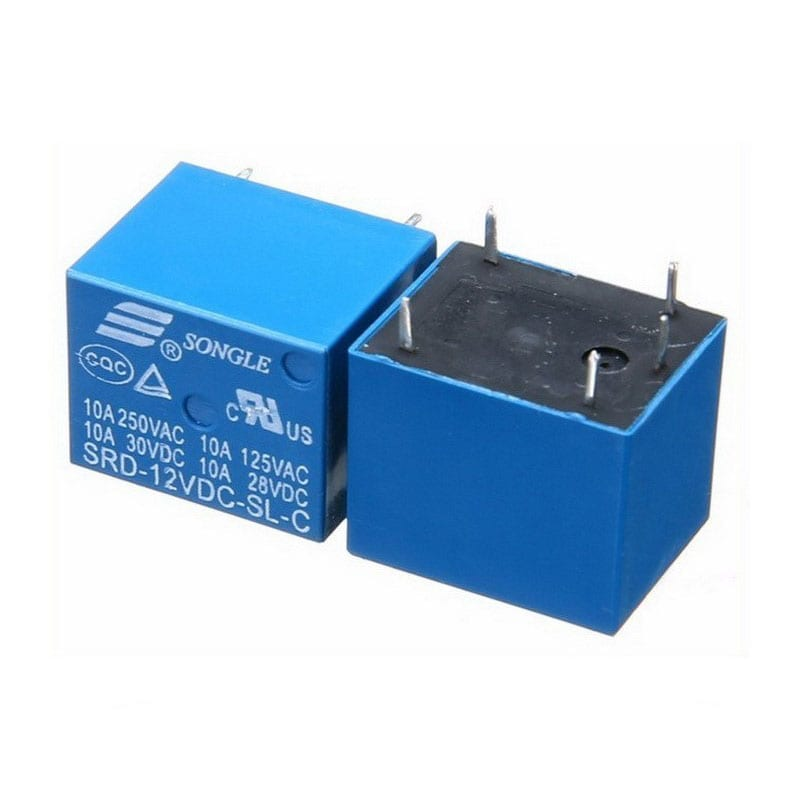
\includegraphics[width=5cm]{Imagenes/Rele-12V.jpg}
     \caption{Relevador}
 \end{figure}

 \subsection{PWM}

La modulación por ancho de pulsos de una señal o fuente de energía es una técnica en la que se modifica el ciclo de trabajo de una señal periódica, estos pulsos varían proporcionalmente
a la amplitud de una señal de entrada.

\begin{figure}[htb]
    \centering
    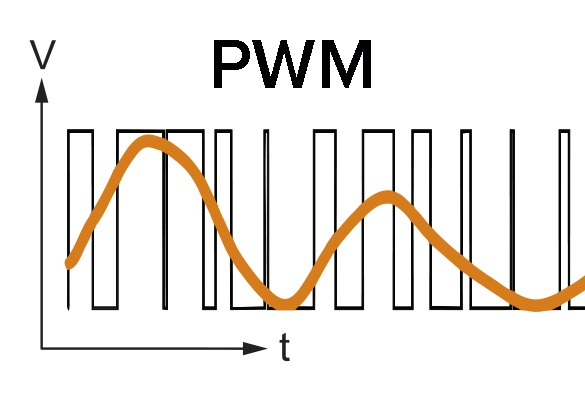
\includegraphics[width=8cm]{Imagenes/PWM.jpg}
    \caption{ Gráfica de la modulación por ancho de pulsos}
\end{figure}

\subsection{Microcontrolador PSOC}

PSoC es la denominación comercial de una familia de microcontroladores programables desarrollada por Cypress Semiconductors. La tarjeta es un sistema configurable
dentro de un chip, el cual reúne periféricas analógicas y digitables configurables, memoria y microcontrolador.

\clearpage

\begin{figure}[htb]
    \centering
    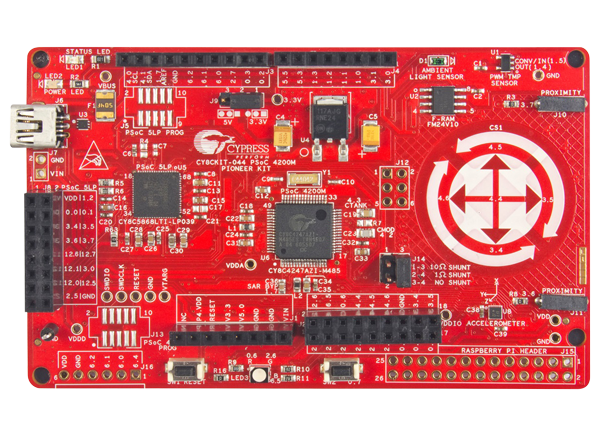
\includegraphics[width=6cm]{Imagenes/PSOC.png}
    \caption{Tarjeta PSoC 4 empleada en esta práctica}
\end{figure}

\section{Instrucciones}

Se pretende desarrollar un circuito que permita modificar el sentido de corriente y su voltaje en un motor DC, para que se puedan apreciar los cambios de dirección y velocidad 
en el mismo. 

\section{Materiales}



\section{Desarrollo}



\section{Resultados}


\section{Conclusiones}


\bibliographystyle{alpha}


\end{document}